\documentclass[a4paper,10pt]{article}
\usepackage[utf8x]{inputenc}
\usepackage{url}
\usepackage{graphicx}
\usepackage{array}

%opening
\title{Etat de lard}
\author{Aurélien Barbotin Pierre David Benjamin Michelland Youna le Vaou}

\begin{document}

\maketitle

\section{État de l'art}
\subsection{Imagerie satellite hyperspectrale}

Jusqu'à récemment, la principale source d'images satellite hyperspectrales exploitées par les scientifiques étaient les satellites MODIS (Moderate-Resolution Imaging SpectroRadiometer). Ces deux satellites, lancés par la NASA en 1999 et 2002, imagent l'intégralité de la surface de la terre tous les deux jours. Ces satellites sont capables de mesurer 36 bandes fréquentielles avec trois résolutions différentes : 250m, 500m et 1000m\cite{nasa}. L'objectif de cette mission est de ``jouer un rôle vital dans le développement de modèles globaux, validés et interactifs de systèmes terrestres capables de prévoir des changements globaux avec suffisamment de précision pour aider les décideurs politiques à prendre des décisions avisées concernant la protection de notre environnement.''

Ces données ont ainsi pu servir à analyser la qualité de l'air au niveau du sol et, entre autres, d'en déduire la présence d'évènements exceptionnels comme des feux de forêt ou du brouillard\cite{airSurv}. A l'aide d'indices comme le NDVI (normalized difference vegetation index) calculés à partir de données multispectrales, il est possible d'établir la présence ou l'absence de végétation dans une zone. En effet, les plantes chlorophyliennes absorbent fortement la lumière rouge et réfléchissent la lumière proche infrarouge : la différence normalisée d'intensité entre ces deux bandes correspond à l'indice NDVI dont une valeur proche de 1 indique la présence de végétation, et une valeur proche de 0 son absence. De multiples applications, comme l'étude de la désertification de zones dues à l'activité humaine\cite{desert} ont dores et déjà été mises en évidence. Il a également été possible d'établir une classification des sols \cite{mapping} en différentes zones (forêt, villes, désert, mer etc.)

La faible résolution des données MODIS ne permet en revanche pas de discerner des détails comme des cours d'eau ou des habitations, et des données plus précises sont donc nécessaires pour obtenir des classifications plus exactes. 

Dans le cadre du projet \textit{Copernicus} d'observation de la Terre, l'agence spatiale européenne (ESA) développe en ce moment les missions Sentinel. Chacune de ces missions consiste en une paire de satellite en orbite autour de notre planète, récoltant des données sur la surface et l'atmosphère. Ainsi, les satellites Sentinel 2 (Sentinel 2-A lancé le 23 juin 2015 et 2-B dont le lancement est prévu pour la seconde moitié de 2016)\cite{sent2} récoltent des données hyperspectrales sur 13 bandes de fréquence : 4 bandes avec une résolution de 10m et 9 avec une résolution de 60m.

Les données Sentinel 2 étant très récentes, nous faisons partie des premiers à les analyser et aucun article à leur sujet n'a encore été publié à notre connaissance. Leur analyse et leur classification relève donc de la recherche.

\section{Résultats}
Dans un but de répétabilité, nous avons testé et optimisé toutes nos méthodes de machine learning sur une unique image hyperspectrale (dont une vue en RGB est donnée en figure \ref{fig:veniseRGB}).
\begin{figure}
  \centering
    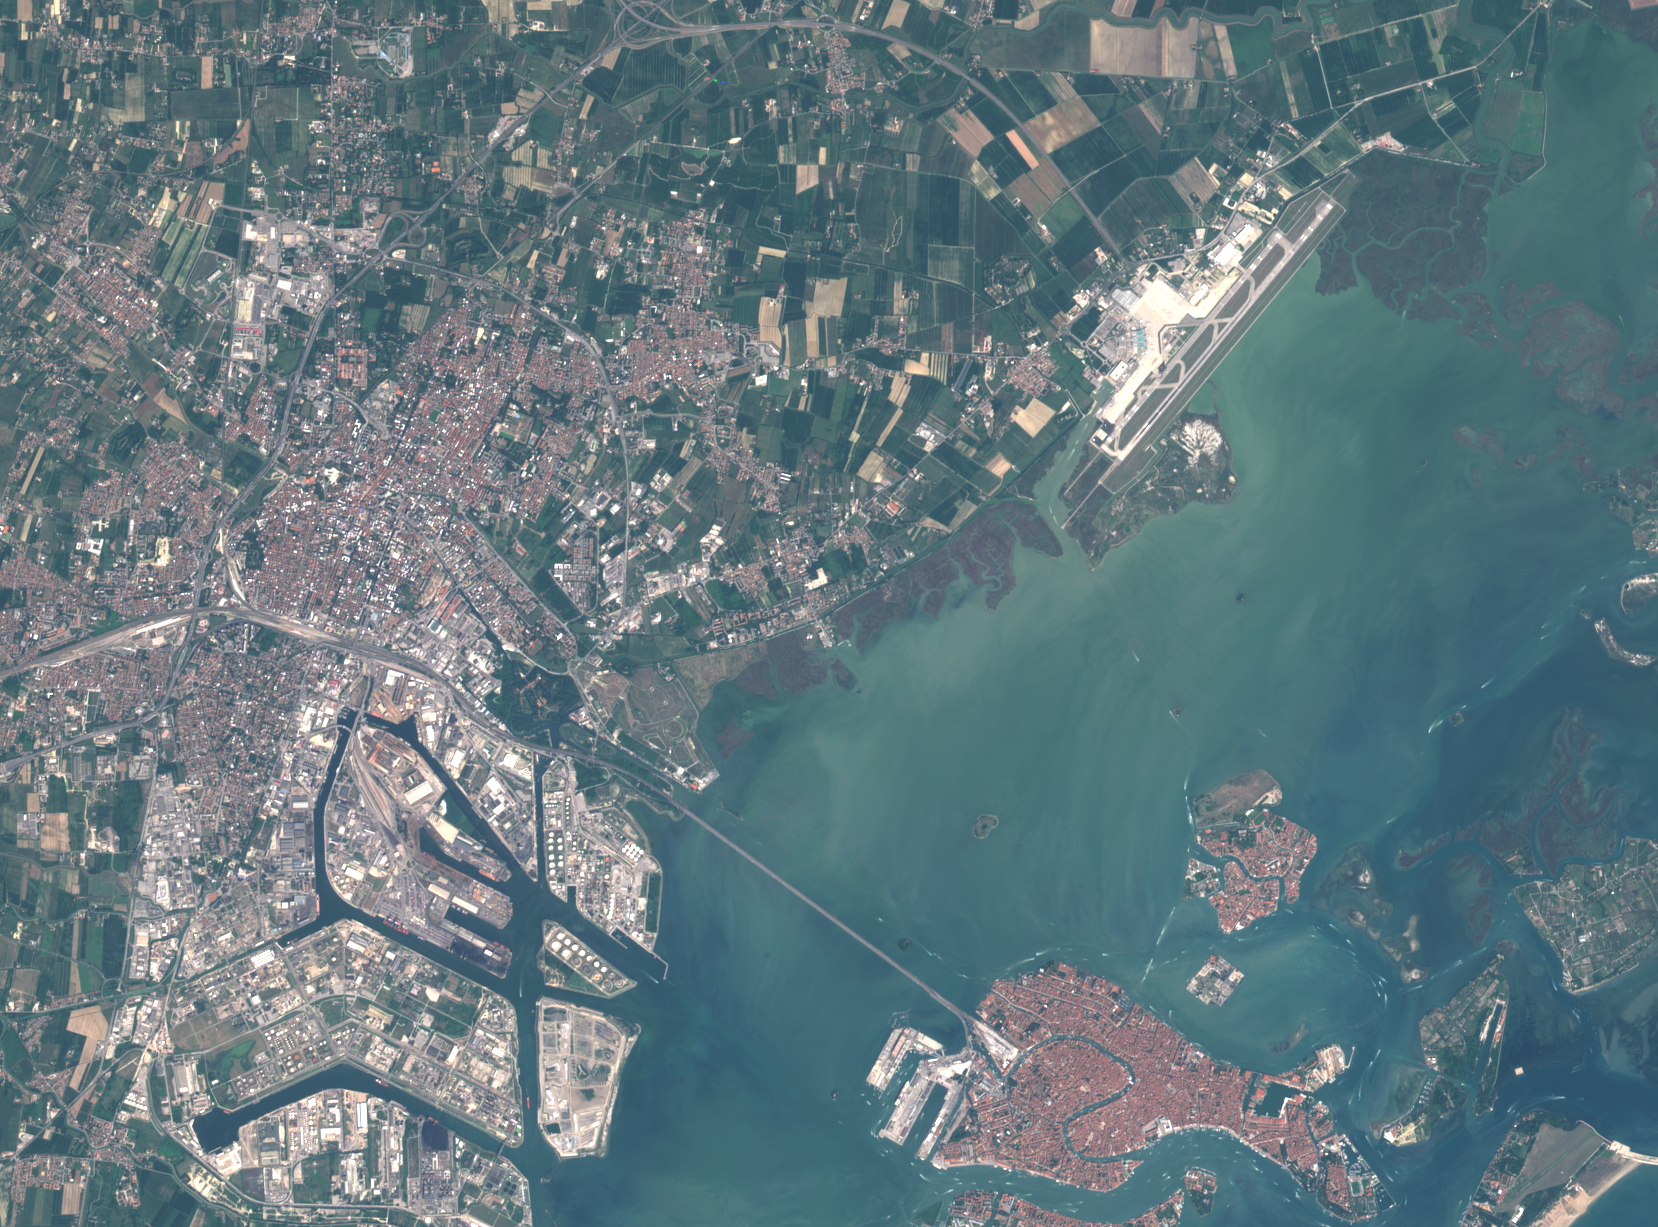
\includegraphics[width=0.5\textwidth]{venise}
  \caption{Image hyperspectralde de Venise qui nous a servi de référence (vue en RGB)}
  \label{fig:veniseRGB}
\end{figure}
Le résultat d'une classification est une image RGB dont la couleur de chaque pixel représente la classe à laquelle il appartient selon l'algorithme. Par exemple, dans une image résultat, un pixel bleu correspond à un point indentifé par l'algorithme comme étant de l'eau. Notre code couleur est résumé dans le tableau \ref{table:codeCouleur}.
\begin{figure}
 \begin{center}
  \begin{tabular}{|c|c|}
    \hline
    Nature du terrain & couleur \\
    \hline
  Champ & Vert \\
  Ville &  Rouge \\
  Eau &  Bleu \\
  Boue & Marron \\
    \hline
  \label{table:codeCouleur}
  \end{tabular}
\caption{Code couleur des images produites par machine learning.} 
\end{center}
\end{figure}
Estimer la qualité d'un classificateur revient à estimer la qualité de l'image résultante. Pour cela, deux méthodes s'offrent à nous: la première numérique, consiste à calculer la matrice de confusion de chaque classificateur comme expliqué INSERER ICI OU CEST EXPLIQUE. L'autre méthode consiste à estimer à l'oeil la correspondance entre les prédictions de nos algorithmes et la réalité (les zones de référence étant elles-mêmes choisies à l'oeil, ce critère n'est pas plus mauvais que l'autre). Pour immédiatement visualiser cette correspondance, nous superposons l'image de base avec l'image résultante en transparence, comme par exemple sur la figure \ref{fig:veniseLSE}.

\subsection{classificateur linéaire}
\label{lineaire}
La première classification que nous testée est aussi la seule que nous avons entièrement implémentée nous mêmes. Il s'agit de classification à l'aide d'un classificateur linéaire. Les résultats obtenus sont encourageants, avec une première classification qui à première vue correspond à la répartition réelle des trois classes étudiées (figure \ref{fig:veniseLSE} avec la matrice de confusion correspondante \ref{table:confknn}).

\begin{figure}
  \centering
    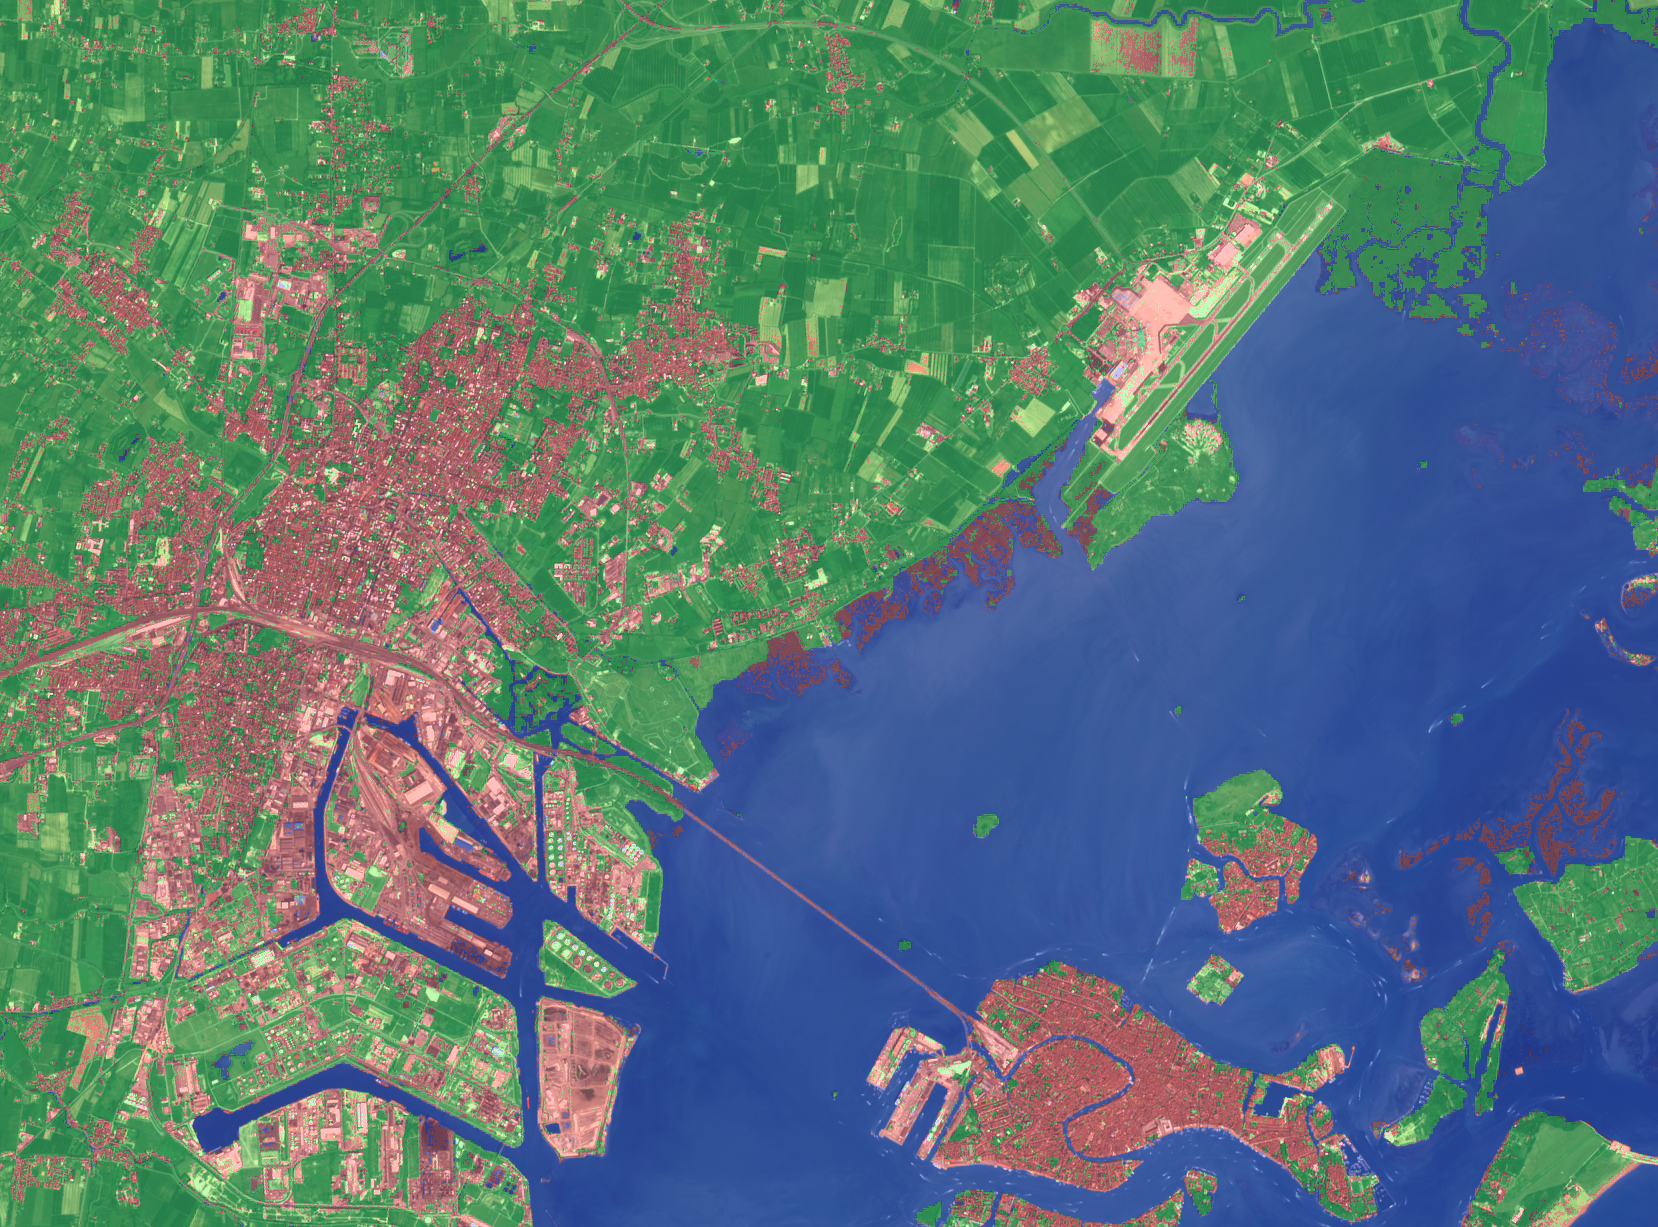
\includegraphics[width=0.5\textwidth]{veniseLSE}
  \caption{Résutat de classification avec un classificateur linéaire}
  \label{fig:veniseLSE}
\end{figure}

\begin{figure}
\begin{center}
 \begin{tabular}{|c|c|c|c|c|}
  \hline
  Nature du terrain & Ville & Champ & Eau & Rappel \\
  \hline
Ville & 5309   &   878    &   15 & 0.856014 \\
Champ & 1296   &  9832     &   0  & 0.883537 \\
Eau &  2   &     0  &   6350 & 0.999685 \\
Précision & 0.803542  & 0.918021 & 0.997643 & 0.907483 \\
  \hline
\end{tabular}
\end{center}
\caption{Matrice de confusion de la classification linéaire}
\label{table:confknn}
\end{figure}

La précision totale de cette méthode est de 90.7\%. On peut constater que l'eau est très bien classifiée, et que les erreurs proviennent majoritairement de confusions entre les champs et la ville.

\subsection{LDA: Analyse linéaire de discriminant}
La classification LDA, pour Linear Discriminant Analysis (Analyse linéaire de discriminant) suppose une distribution gaussienne des points au sein de chacune des classes. Or, nous avons choisi des polygones de manière à ce qu'ils contiennent le moins de points possibles, le plus représentatifs possibles, afin de diminuer les temps de calcul. Ce faisant, on n'a pas pris un échantillon continu de points et l'approximation gaussienne est difficilement valable, ce qui explique les mauvais résultats obtenus, en particulier sur les zones de ville.
\begin{figure}
  \centering
    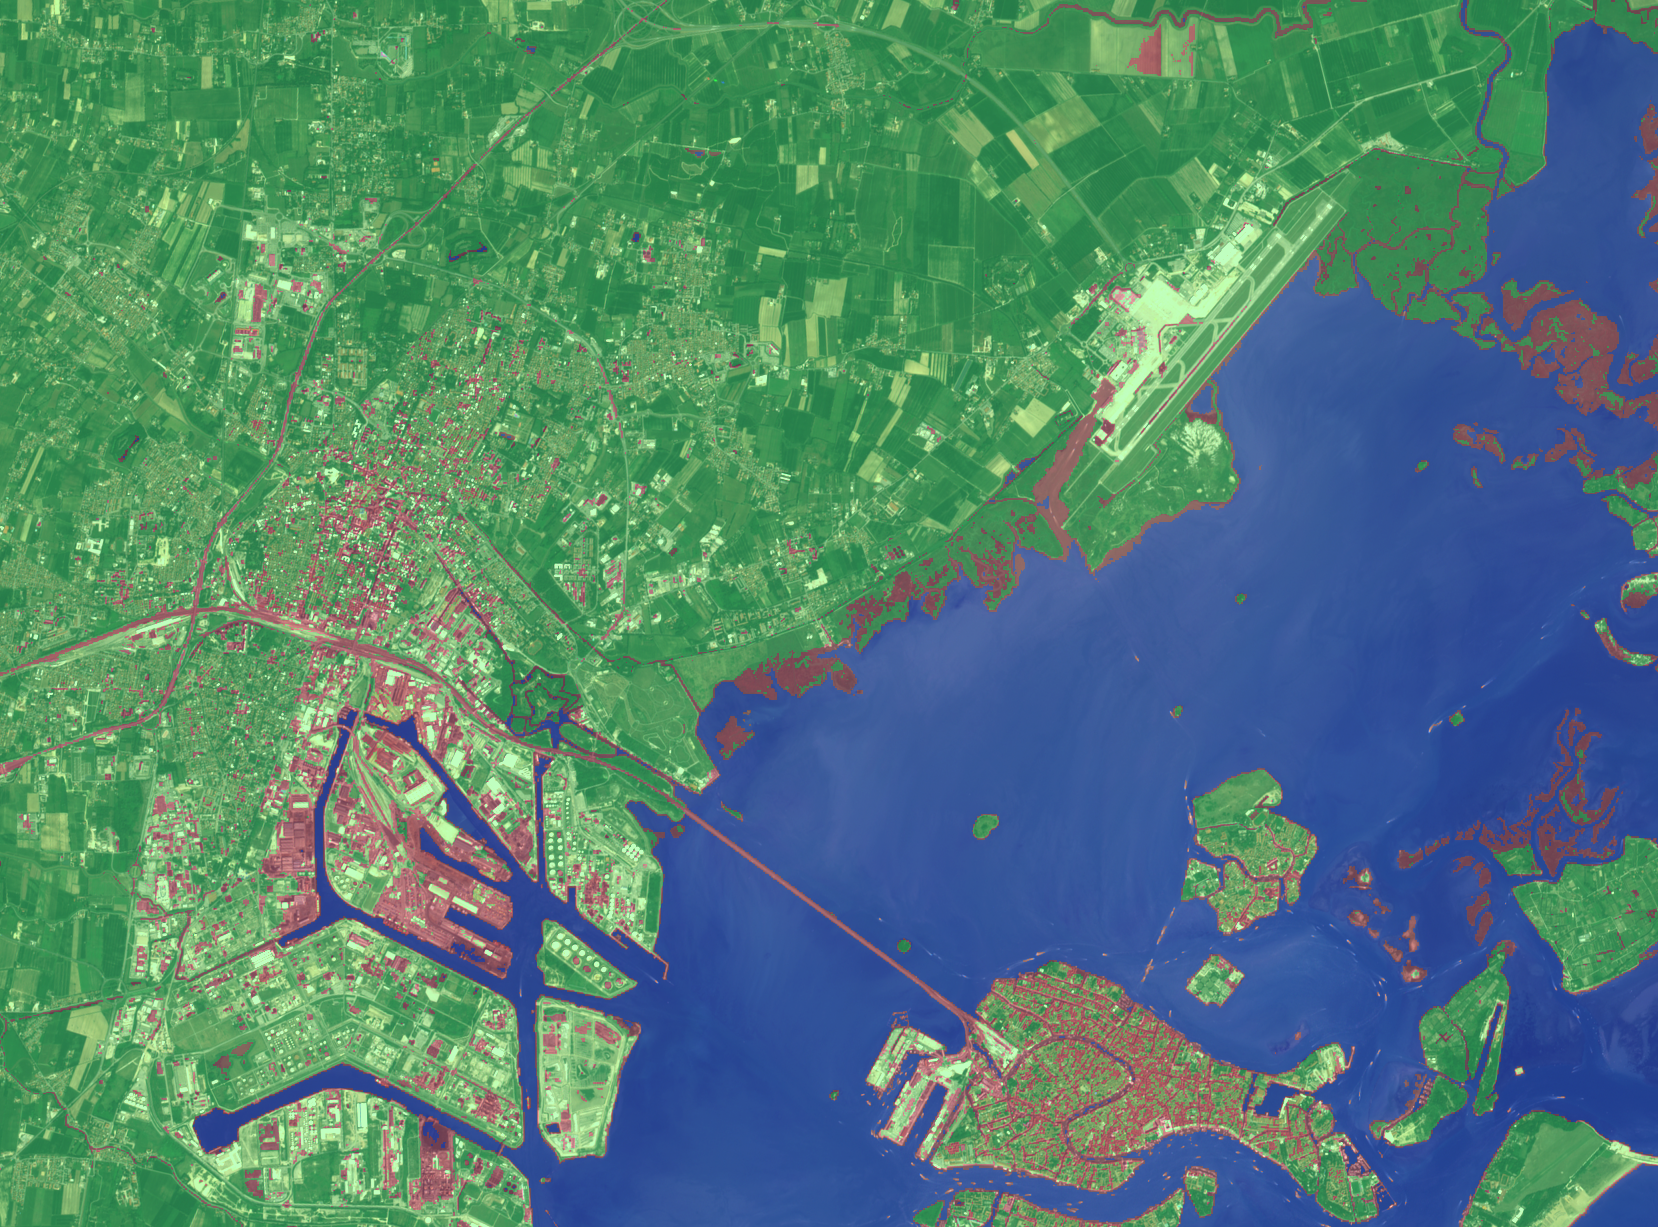
\includegraphics[width=0.5\textwidth]{venise+LDA}
  \caption{Résutat de classification avec une analyse linéaire de discriminant}
  \label{fig:veniseLDA}
\end{figure}

\begin{table}
\begin{center}
 \begin{tabular}{|c|c|c|c|c|}
  \hline
  Nature du terrain & Ville & Champ & Eau & Rappel \\
  \hline
Ville & 2026  &   4176  &      0 & 0.326669 \\
Champ & 675  &  10453   &     0 & 0.9393427 \\
Eau &  0    &    0  &   6352   &     1 \\
Précision & 0.750093 & 0.71454  &      1 & 0.795161\\
  \hline
\end{tabular}
\end{center}
\caption{Matrice de confusion de l'analyse avec discriminant linéaire }
\label{table:veniseLDA}
\end{table}
    
     

\subsection{méthode knn:k-nearest-neighbours ou k plus proches voisins}
La méthode des k-nearest neighbors présente des résultats intéressants, et nous avons obtenu une classification très précise avec cette méthode. Nous avons testé cette méthode avec différentes valeurs de k (1 à 10, 20, 200) et il s'est avéré que les plus faibles valeurs de k sont aussi celles qui fournissent la meilleure exactitude (voir figure \ref{fig:kNN}), ce qui nous laisse penser que les points sont naturellement bien séparés. Nous avons donc choisi de faire notre classification avec la valeur du paramètre k=1. Les résultats obtenus sont montrés sur la figure \ref{fig:1NN} et le tableau \ref{table:1NN}.

\begin{table}
\begin{center}
 \begin{tabular}{|c|c|c|c|c|}
  \hline
  Nature du terrain & champ & ville & eau & Rappel \\
  \hline
Champ & 9929 & 71 & 	0 &	99.29 \\
Ville & 540 &	9460 &	0 &	94.6 \\
Eau &  0 &	0 &	10000 &	100 \\
Précision & 99.29 & 94.6 & 100 & 97.96 \\
  \hline
\end{tabular}
\end{center}
\label{table:1NN}
\caption{Matrice de confusion de l'algorithme de 1-plus proche voisin.}
\end{table}

\begin{figure}
  \centering
    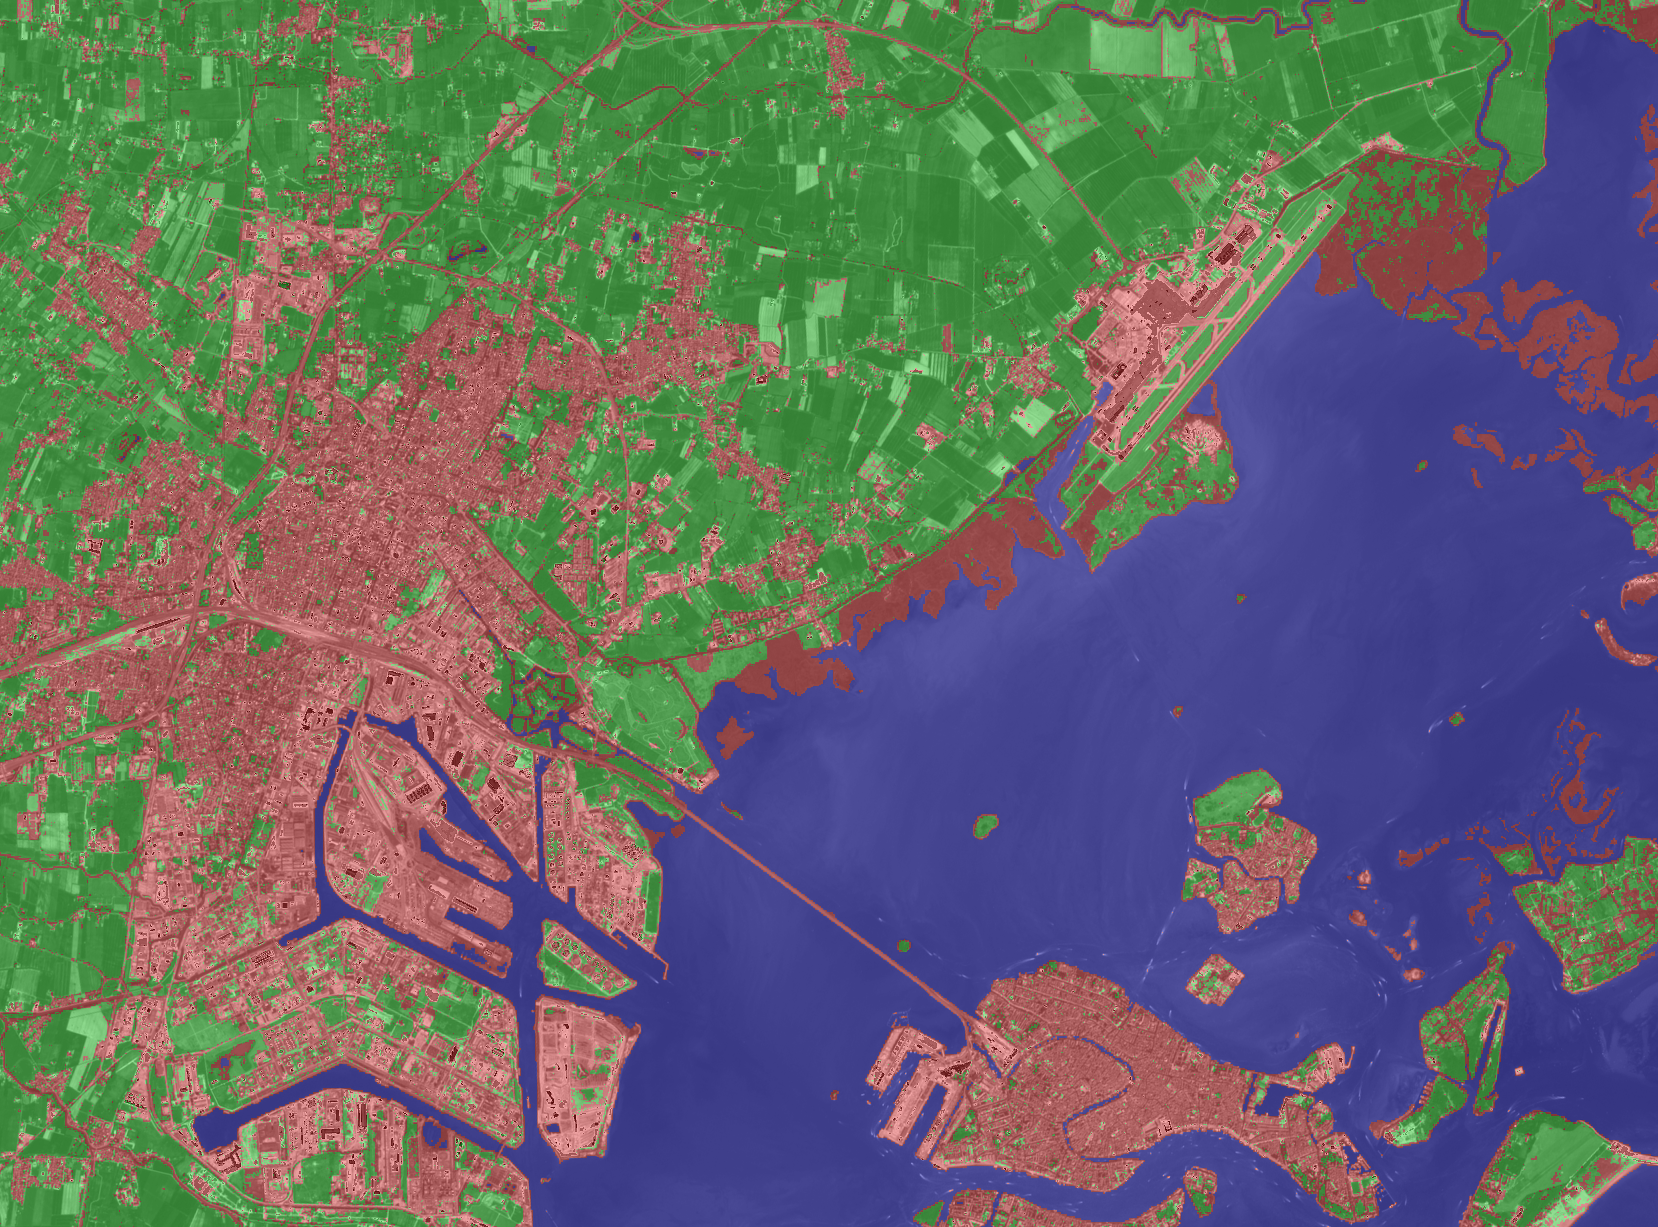
\includegraphics[width=0.5\textwidth]{resultat1NN}
  \caption{Résutat de classification avec la méthode du 1-plus proche voisin}
  \label{fig:1NN}
\end{figure}

On observe également une exactitude en moyenne moindre pour les valeurs paires de k, par rappor aux valeurs impaires : cela vient du fait que nous n'avons pas mis en place de système de vote en cas de conflit. En effet, si la moitié des voisins appartiennent à une classe, et l'autre moitié appartient à une autre classe, le système choisit aléatoirement dans quelle classe placer le pixel. Il est possible de remédier à cela en choisissant un système de vote adapté (par exemple, en cas d'égalité, calculer la distance à chaque voisin et choisir la classe pour laquelle la distance totale est la plus faible.)

\begin{figure}
  \centering
    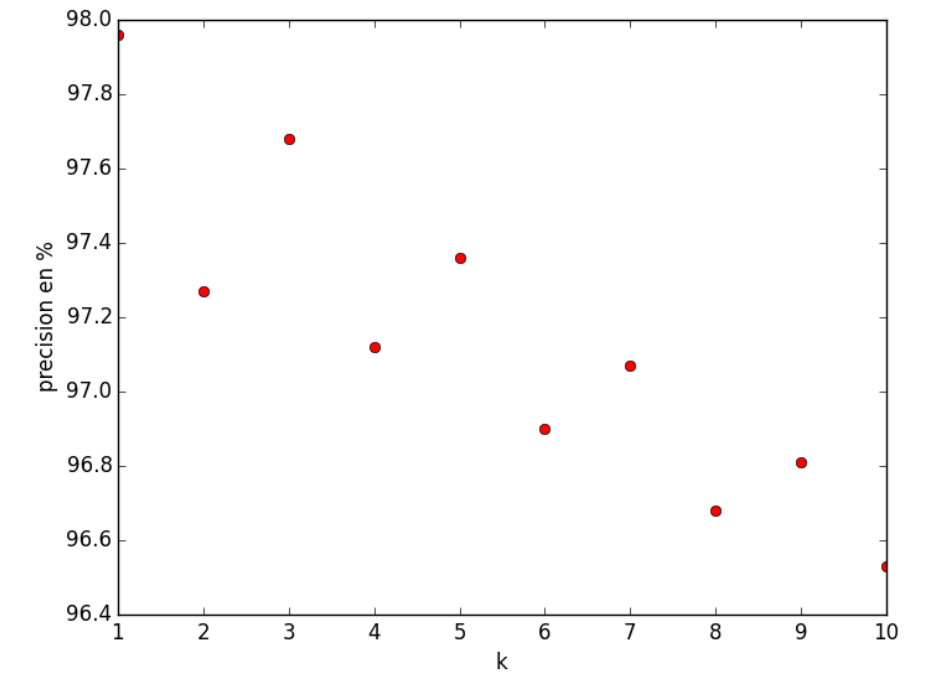
\includegraphics[width=0.5\textwidth]{influencek.png}
  \caption{Influence du paramètre k sur l'exactitude de l'algorithme.}
  \label{fig:kNN}
\end{figure}


\subsection{Support Vecteur Machine}
Cette méthode utilise deux métaparamètres : C et $\gamma$. Afin d'optimiser l'apprentissage et la classification de notre image, il faut donc trouver les métaparamètres idéaux. Pour cela, on fait un ensemble de validations croisées dans lequel on sépare notre jeu de données en 5, 4 parts servant à l'apprentissage et la dernière part au test. On fait ce test 100 fois pour 100 couples de valeurs (C,$\gamma$), et le jeu de paramètres obtenant le meilleur score de précision lors de la validation croisée correspondaux paramètres que l'on utilisera. Afin de déterminer d'un seul coup d'oeil si l'on a trouvé un set de paramètres optimal, on représente les résultats des différentes validations croisées sur une courbe en deux dimensions (figure \ref{fig:crossMap}).

\begin{figure}
  \centering
    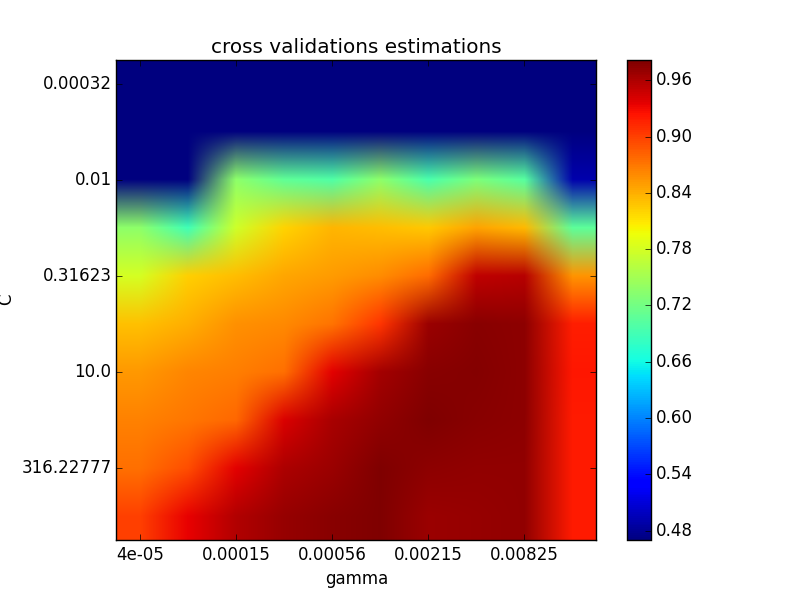
\includegraphics[width=0.5\textwidth]{crossValLog}
  \caption{Scores obtenus pouf 100 validations croisées avec différents couples de paramètres (C,$\gamma$). La couleur d'un point correspond à la précision moyenne de l'algorithme pour le couple (C,$\gamma$) qui lui sert de coordonnées. Les axes sont en échelle logarithmique.}
  \label{fig:crossMap}
\end{figure}

Cette figure qu'en effet, la précision de l'algorithme dépend du choix judicieux des métaparamètres. Le meilleur choix de métaparamètres dans notre cas est le couple (C,$\gamma$)=(1,$ 10^{-3}$). Nous obtenons alors l'image \ref{fig:veniseSVM} et la matrice de confusion \ref{table:SVC}.

\begin{table}
\begin{center}
 \begin{tabular}{|c|c|c|c|c|}
  \hline
  Nature du terrain & Ville & Champ & eau & Rappel \\
  \hline
Ville & 9867 & 133 & 	0 &	98.67 \\
Champ & 159 &	9841 &	0 &	98.41 \\
Eau &  38 &	0 &	9962 &	99,62 \\
Précision & 98.04 & 98.6 & 100 & 98.9 \\
  \hline
  \end{tabular}
\end{center}
\label{table:SVC}
\caption{Matrice de confusion de l'algorithme de Support Vecteur Machine.}
\end{table}

\begin{figure}
  \centering
    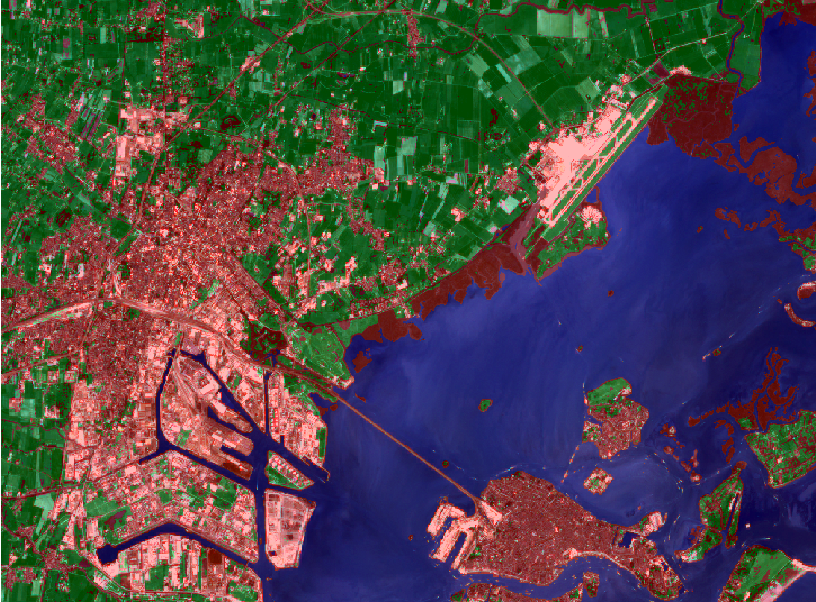
\includegraphics[width=0.5\textwidth]{veniseSVM}
  \caption{Résutat de classification avec le support vecteur machine.}
  \label{fig:veniseSVM}
\end{figure}

\subsection{Conclusion}
La première conclusion que nous pouvons tirer de notre travail est que les méthodes de machine learning que nous avons testées donnent pour la plupart des résultats très satisfaisants. Le support vecteur machine en particulier nous fournit une exactitude de 98.9\% avec trois classes. Il est d'usage de prétraiter les données pour calculer des indices comme l'index de végétation différentiel normalisé (NDVI)\cite{NDVI}:
\begin{equation}
NDVI=\frac{NIR-VIS}{NIR+VIS}
\end{equation}
Où NIR correspond à l'intensité lumineuse dans le proche infrarouge et VIS dans le rouge. Une valeur de cet indice proche de 1 indique la présence de végétation, une valeur négative indique des nages ou l'absence de végétation. Dans notre cas, les images multispectrales fournissent suffisamment d'informations par elles-mêmes pour classifier les sols avec précision sans passer par cet indice.

L'un des objectifs de notre projet étant de déterminer des principes généraux pour la classification et l'exploitation des données Sentinel-2, nous avons cherché à comparer les résultats obtenus pour différents classificateurs. Nous avons d'abord cherché à comparer à l'oeil ces méthodes en cherchant des différences sur les images obtenues, comme sur la figure \ref{comparaison}.

\begin{figure}
  \centering
    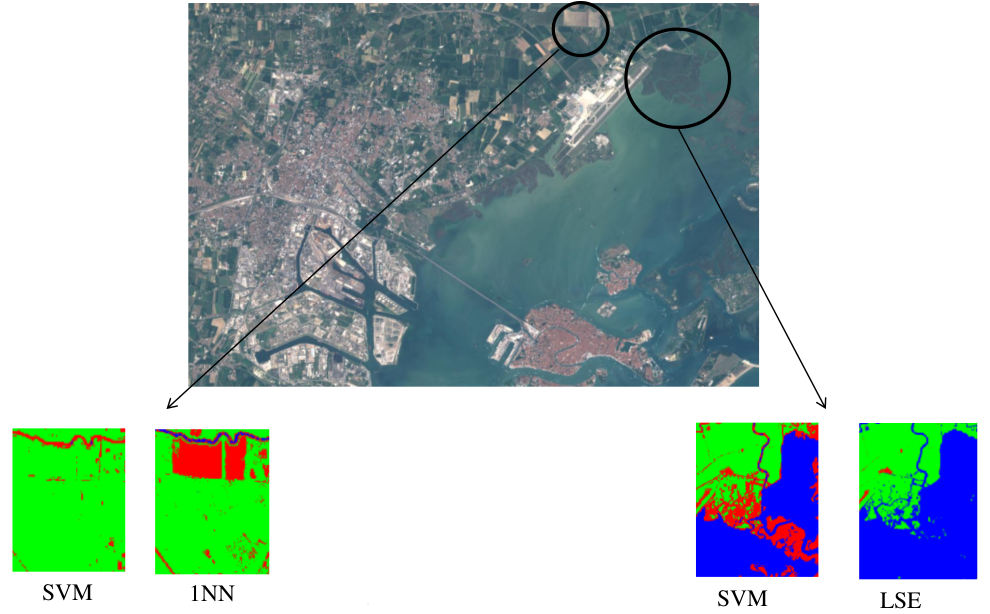
\includegraphics[width=0.5\textwidth]{comparaison}
  \caption{Comparaison des classifications obtenues avec différentes méthodes.}
  \label{fig:comparaison}
\end{figure}
Cependant, ces comparaisons à l'oeil ne permettent pas d'identifier formellement un critère meilleur que l'autre. Nous avons donc utilisé un critère numérique : l'exactitude, qui permet de quantifier la qualité de nos classifications et ainsi de les comparer. Les résutats sont résumés dans le tableau \ref{table:comp}. On peut constater que selon ces résultats, le support vecteur machine (SVM) offre les meilleurs résultats et semble donc le classificateur le plus adapté à notre problème de classification à trois classes. Il serait nécessaire de faire des tests similaires sur d'autres zones pour confirmer ou infirmer cette observvation, cependant cela sort du cadre de notre projet.

\begin{table}
\begin{center}
 \begin{tabular}{|c|c|c|c|c|}
  \hline
  type de classification & LDA & LSE & 1NN & SVM \\
  \hline
exactitude & 78.4\% & 90.9\% & 	98.0\% & 99.1\% \\
  \hline
  \end{tabular}
\end{center}
\label{table:comp}
\caption{Comparaison des différents classificateurs}
\end{table}

Nous avons également démontré que chacune des 12 bandes spectrales est nécessaire dans la classification, puisque la perte de l'une d'entre elles entraîne une baisse significative de l'exactitude comme on l'a vu dans le paragraphe \ref{lineaire}. Nous avons étudié l'influence de ce paramètre en étudiant l'exactitude d'un classificateur avec les 12 bandes, puis en en retirant. Les résultats obtenus sont présentés en figure \ref{fig:nBandes}.

\begin{figure}
  \centering
    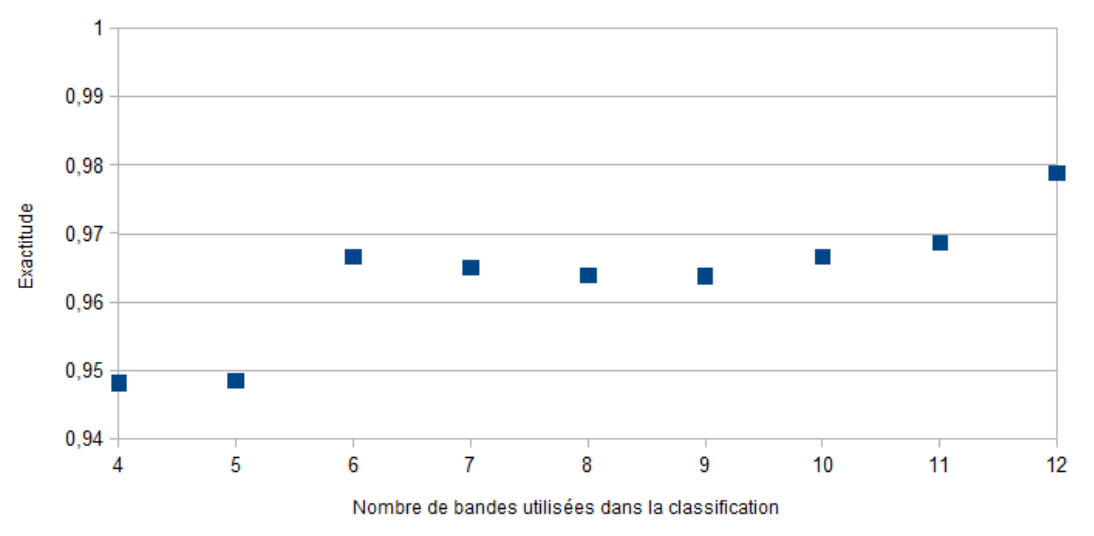
\includegraphics[width=0.5\textwidth]{nBandes}
  \caption{Influence du nombre de bandes spectrales sur la qualité de classification d'une méthode des 1 plus proches voisins.}
  \label{fig:nBandes}
\end{figure}

\subsection{Limites et améliorations}
Nous avons constaté que la boue le long des côtes n'est pas toujours reconnue de la même manière par nos algorithmes: parfois champs, parfois ville, ils ne correspondent à aucune de nos trois classes. Il est en effet rare en apprentissage automatique d'utiliser seulement trois classes. Nous avons donc rajouté une classe ``boue'' et testé certaines de nos classifications dessus, en particulier le Support Vecteur Machine. Le résultat est donné en figure \ref{fig:SVM4Cl}. La boue est bien classifiée mais l'introduction de cette 4e classe entraîne l'apparition de faux positifs, en particulier dans les champs dont la réponse spectrale est proche.
\begin{figure}
  \centering
    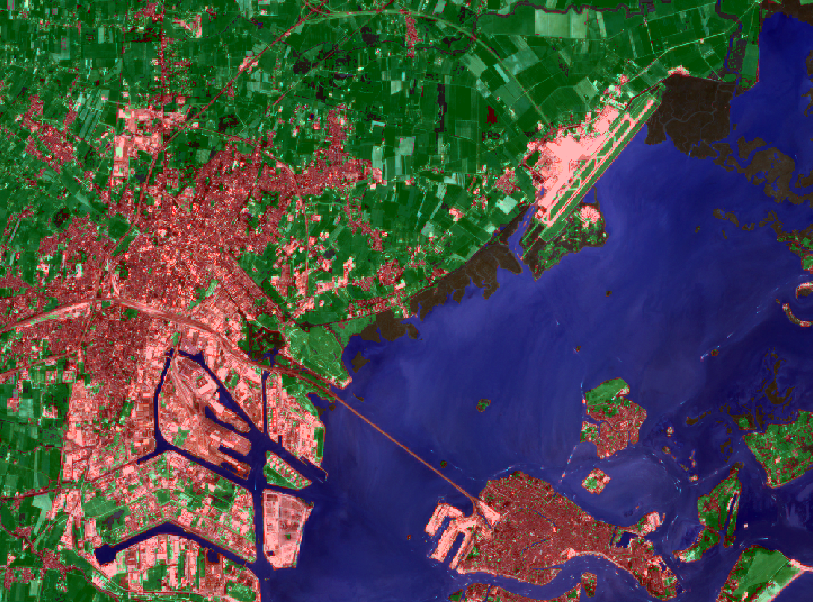
\includegraphics[width=0.5\textwidth]{SVM4Classes}
  \caption{Résutat de classification de 4 classes avec le support vecteur machine.}
  \label{fig:SVM4Cl}
\end{figure}

Plusieurs méthodes s'offrent à nous pour améliorer ce résultat de classification: la plus simple, appelée \textit{whitening} (blanchissement, en français) consiste à centrer chaque bande spectrale sur sa moyenne et à la dilater proportionnellement à son écart-type. Cette méthode renormalise les distributions et permet une meilleure classification.

Il est également possible d'ajouter encore plus d'informations, en utilisant les données de satellites Sentinel-1 qui sont des images radar. Une dernière méthode tout juste mise au point par notre tuteur N. Brodu consiste à améliorer la résolution des bandes spectrales de plus faible résolution en inférant leur valeur à partir des bandes à plus haute résolution. Ces méthodes ont prouvé leur efficacité sur les données MODIS et pourraient apporter un supplément d'information sur les données Sentinel-2 également.

Enfin, les données sentinel-2 étant toutes nouvelles, peu de scènes sont à notre disposition. Nous nous sommes concentrés pendant ce projet sur une zone précise dans un but de répétabilité. Nous avons essayé de classifier des zones différentes comme présenté en figure \ref{fig:zone2},cependant ce travail n'a été qu'esquissé et sort du cadre de notre projet.

\begin{figure}
  \centering
    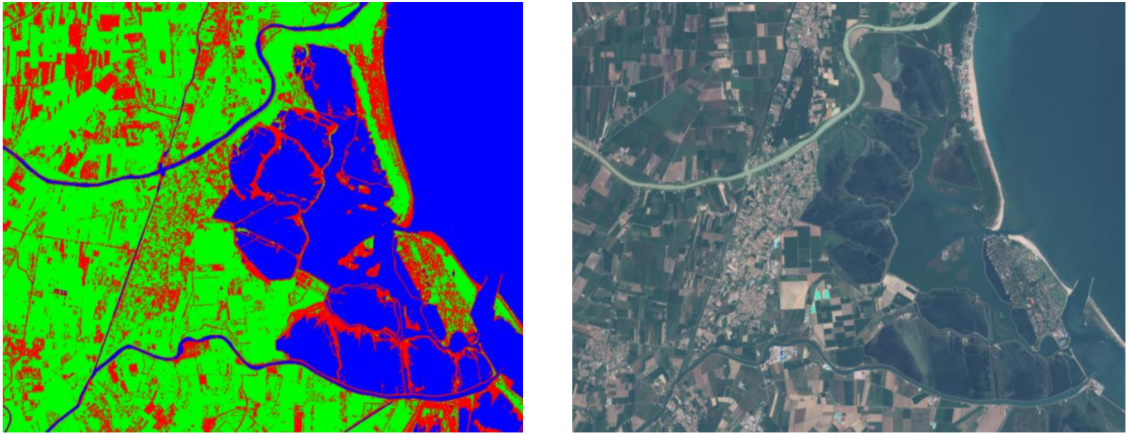
\includegraphics[width=0.7\textwidth]{zone2}
  \caption{Résutat de classification d'une autre zone en Italie du nord}
  \label{fig:zone2}
\end{figure}

\bibliography{Biblio}
\bibliographystyle{plain}
\end{document}
